%!TEX root = ../TTK4900-MHT.tex

\chapter{Radar and AIS preprocessing}\label{chapter:radar-and-ais-preprocessing}
The process from raw radar and \gls{ais} data to target tracks is made up from several processing steps. The aim of this chapter is to give the reader a basic understanding of these steps and their challenges.

\section{Radar preprocessing}
Rotating maritime radars (Figure~\ref{fig:maritime_radar_antenna}) are wide and short, giving them a tall and narrow beam. A ping transmit and receive sequence is carried out for each antenna rotation angle in the radars scan resolution. This gives reflections as signal level in spokes described by polar coordinates, rotation angle and distance. Each spoke has a width determined by the design of the antenna, primarily the width of the antenna, and a number of cells dictated by the discretization and sampling interval of each spoke. The spokes is then run through a detection algorithm, which is filtering adjusting the received signal according to detection setting. The detection algorithm is often built in to the radar system, with both fixed and user adjustable detection parameters.

When displayed on a screen in a vessels, the output from the detection step is viewed and interpreted by the operators. In an automated scenario with autonomous vessels, the next step would be to transform the detections from polar vessel body frame to for instance a Cartesian world fixed local frame. Which frame to convert two is a design choice, and can be dependent on use-case, interconnected systems and performance requirements. This transformation is strongly dependent on knowing the position and attitude of the vessel at each spoke sampling time, which is fed from the vessels navigation system.

With all the spoke resolution cells converted to a world-fixed Cartesian coordinate system, it is desirable to remove land reflections if any. This step is dependent on highly detailed digital maps of the area in question, and is commercially available for most of the world. Since maps have both offsets and inaccuracies to some extent, a cleaner land masking can be accomplished by dilating the coastline. This is in may situations acceptable since the vessels will never be that close to shore, and any targets masked away is in a region out of interest.

The last step in the radar processing chain is to convert a point cloud into measurements, as one target will in most cases fill multiple resolution cells and therefore it does not yield good result to send all cells with detection forward as measurements. This clustering of the detections also need to take into consideration the assumption that each target maximum generates one measurements. This leads to clustering algorithms that assumes that detections closely spaced are originating from the same target, and thus should be one measurement. There is many clustering algorithms available to solve this problem, some builds graphs with vertices between neighbouring detections given a neighbour criterion, some estimates the number of clusters and optimizing the detections into this number of clusters~\cite{Mahmuddin2010,Pelleg2000}. When a set of detections are clustered, their respective measurement is calculated as the centroid of the detections, which would be weighted by their signal strength if available. These measurements are sent to the tracking module. 

\section{AIS preprocessing}~\label{sec:ais_preprocessing}
\Gls{ais} does not suffer from the association uncertainty, clutter and low accuracy like radar measurement. It does however have some issues caused by suboptimal or erroneous transmitter implementation, transmission collision caused by \gls{tdma} leading to ID (\gls{mmsi}) swaps, and delayed messages leading to out of order reception. In order to remove most of these errors, it is desirable to filter the incoming \gls{ais} messages before sending them to the tracking module.

\subsection{Out-of-order filtering}
All \gls{ais} messages are stamped with the \gls{utc} of transmission, and `frequently arrive out-of-order'~\cite{Wilthil}, illustrated in Figure~\ref{fig:out_of_order_ais} stolen from~\cite{Wilthil}.
%Stjålet hardt og brutalt
\begin{figure}[H]
\centering
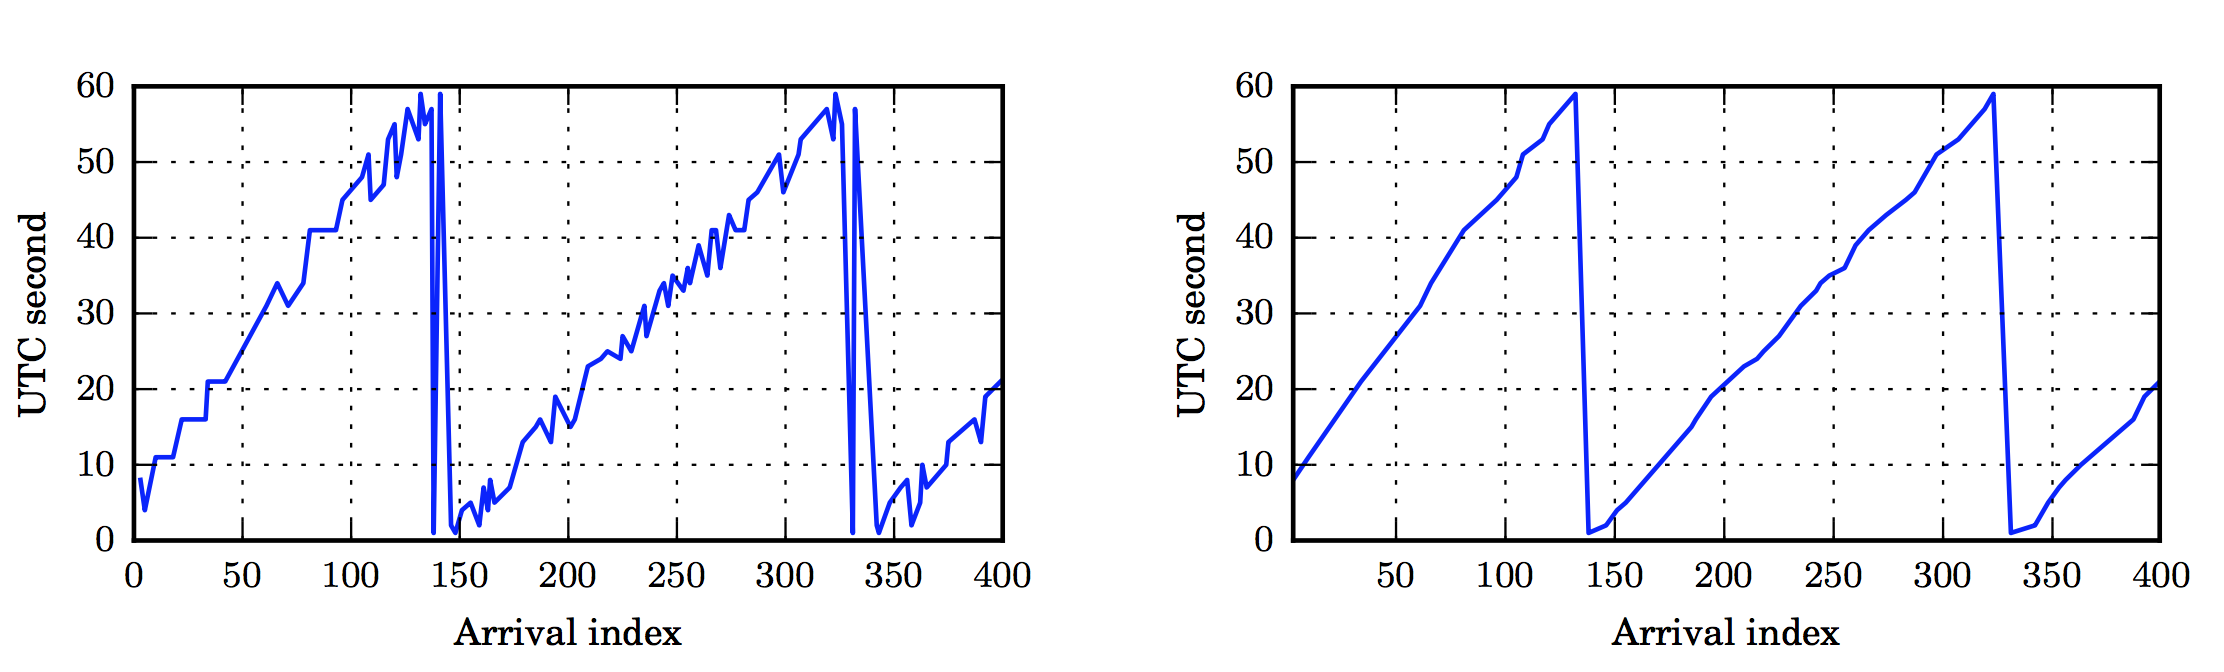
\includegraphics[width = .9\textwidth]{Figures/out_of_order_ais.png}
\caption{Unfiltered and filtered AIS arrival time~\cite{Wilthil}}
\label{fig:out_of_order_ais}
\end{figure}
One of the simplest ways of remedying this issue is to discard all messages with older timestamps that the current newest for each \gls{mmsi}. 

\subsection{ID swap filtering}


\subsection{Synchronization}
All \gls{ais} measurements are buffered from when they are received to the next radar scan. This is a design choice, which in some sense synchronize the AIS to the radar. Since the radar period is much smaller than (or in the best case for the AIS, equal to) the AIS transmit period, this will seldom lead to unused AIS measurements. On the other hand, since the radar period is relative short, the amount of time any AIS position will be predicted forward is typically small enough to not cause uncertainty larger than manageable for the algorithm. 

As will be obvious in Section~\ref{subsec:combined_radar_and_ais_hypotheses}, this prediction is only used for the gating sequence.

